%***************************************************************************
\section{Propagation of the Prior Uncertainties}\label{sec:reflood_prior_uq}
%***************************************************************************

Hence, the \emph{prior uncertainty propagation} step constitutes of generating samples for each model parameter from its prior \gls[hyper=false]{pdf}, 
carrying out a set of \gls[hyper=false]{trace} simulations of the \gls[hyper=false]{feba} model using the sampled parameters, 
and analyzing the results to quantify the uncertainty of the model prediction.

% FEBA Test No. 216 Prior Uncertainty Propagation, TC
\begin{sidewaysfigure}
	\centering
	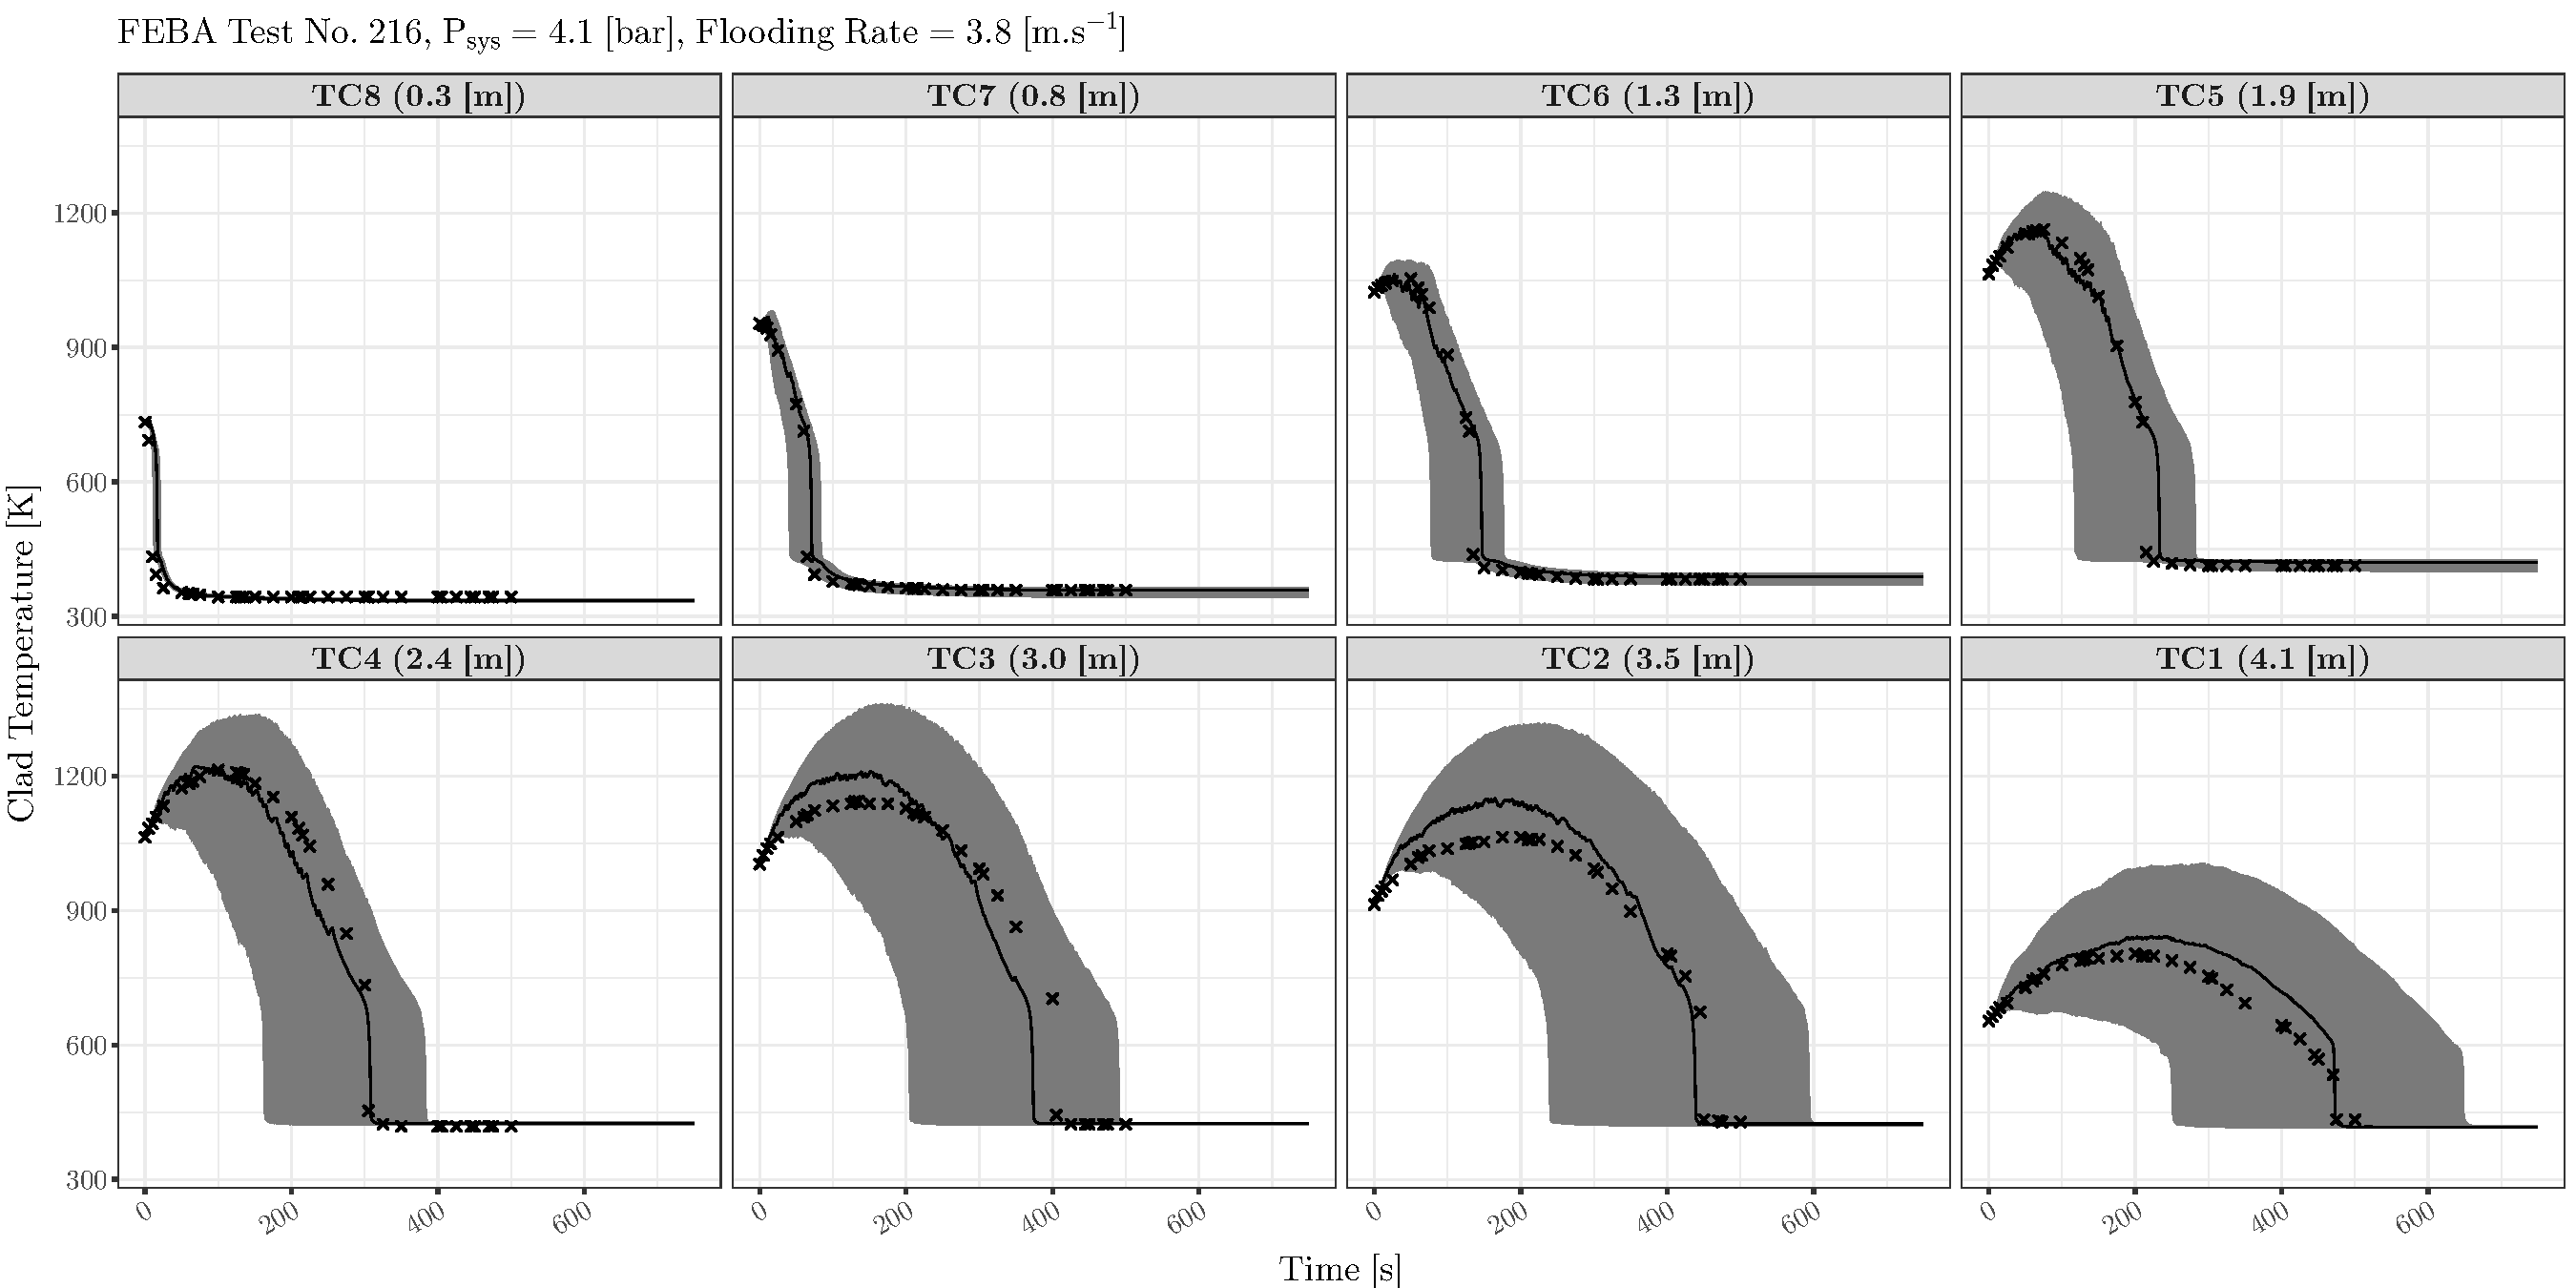
\includegraphics[width=0.90\textwidth]{../figures/chapter2/figures/plotTraceUQPriorTC216}
		\captionof{figure}[Propagation of the $27$ input parameters prior uncertainties on FEBA test No. $216$ for the cladding temperature output ($TC$).]{Propagation of the $27$ input parameters prior uncertainties on FEBA test No. $216$ for the cladding temperature output ($TC$). The uncertainty bound corresponds to the symmetric ($95\%$) probability; solid lines and crosses indicate the simulation with the nominal parameters values and the experimental data, respectively.}
	\label{fig:ch2_plot_trace_uq_prior_tc_216}
\end{sidewaysfigure}


% FEBA Test No. 216 Prior Uncertainty Propagation, DP
\begin{figure}[bth]
    \centering
    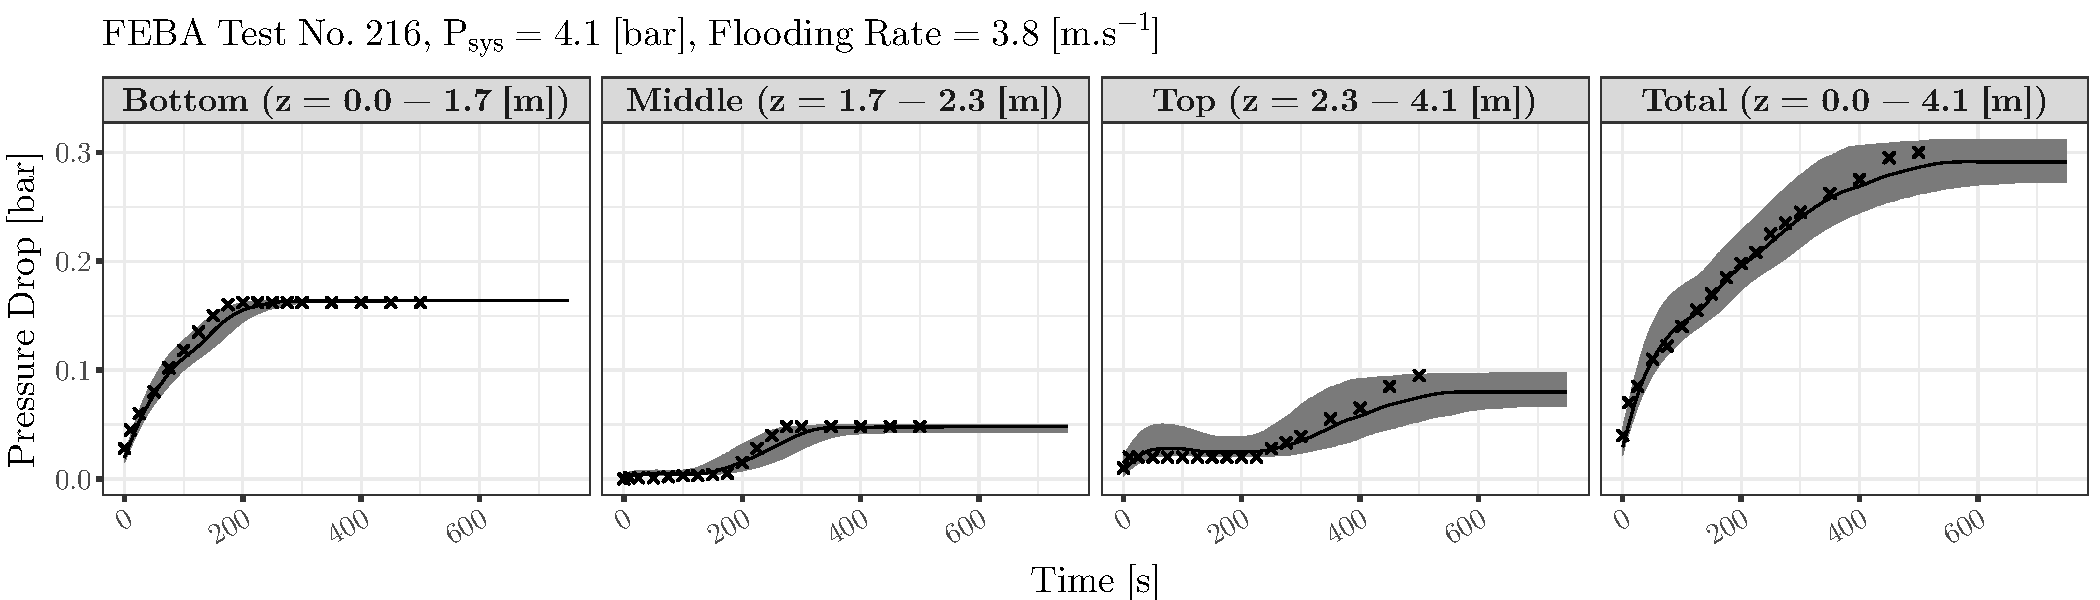
\includegraphics[width=1.0\textwidth]{../figures/chapter2/figures/plotTraceUQPriorDP216}
    \caption[Propagation of the $27$ input parameters prior uncertainties on FEBA test No. $216$ for the pressure drop output ($DP$).]{Propagation of the $27$ input parameters prior uncertainties on FEBA test No. $216$ for the pressure drop output ($DP$). The uncertainty bound corresponds to the symmetric ($95\%$) probability; solid lines and crosses indicate the simulation with the nominal parameters values and the experimental data, respectively.}
    \label{fig:ch2_plot_trace_uq_prior_dp_216}
\end{figure}

\begin{figure}[!bth]
    \centering
    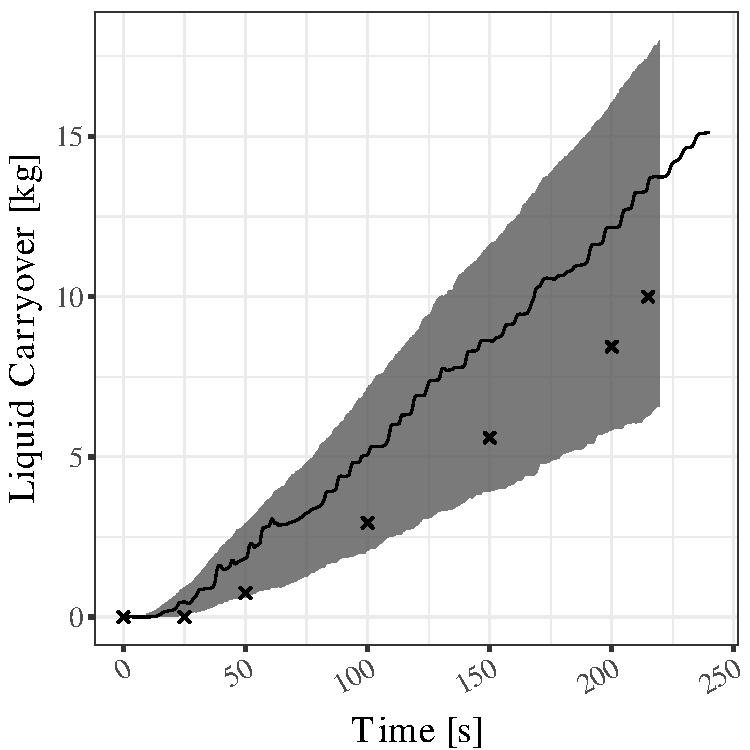
\includegraphics[width=0.5\textwidth]{../figures/chapter2/figures/plotTraceUQPriorCO216}
    \caption[Propagation of the $27$ input parameters prior uncertainties on FEBA test No. $216$ for the liquid carryover output ($CO$).]{Propagation of the $27$ input parameters prior uncertainties on FEBA test No. $216$ for the pressure drop output ($CO$). The uncertainty bound corresponds to the symmetric ($95\%$) probability; solid lines and crosses indicate the simulation with the nominal parameters values and the experimental data, respectively.}
    \label{fig:ch2_plot_trace_uq_prior_co_216}
\end{figure}